% ============================================================
%  PROJECT REPORT — skeleton
%  Compile with pdfLaTeX. Run twice so refs/citations resolve.
% ============================================================
\documentclass[11pt,a4paper]{article}

% ---------- packages ----------
\usepackage[margin=1in]{geometry}   % page margins
\usepackage{amsmath,amssymb}        % equations, symbols
\usepackage{graphicx}               % \includegraphics
\usepackage{float}                  % place figures beside their discussion
\usepackage{booktabs}               % nice tables (\toprule etc.)
\usepackage{siunitx}                % units: \SI{2.598}{}
\usepackage{listings}               % code snippets
\usepackage{caption}
\usepackage{subcaption}             % side-by-side figures
\usepackage[numbers,sort&compress]{natbib}  % citations [1,2]
\usepackage{xcolor}
\usepackage[normalem]{ulem}
\usepackage[hidelinks]{hyperref}    % load LAST
\usepackage[margin=1in]{geometry}
\usepackage{amsmath,amssymb}
\usepackage{graphicx}
\usepackage{caption}
\usepackage[hidelinks]{hyperref}

\graphicspath{{figures/}}           % look for images in figures/

% ---------- shorthand macros (optional but saves typing) ----------
\newcommand{\rs}{R_{\mathrm{s}}}
\newcommand{\rplus}{r_{+}}
\newcommand{\Rt}{\mathbb{R}}
\DeclareRobustCommand{\rev}[2]{{\color{red}\sout{#1} #2}}
\newcommand{\reviewnote}[1]{\par\smallskip\noindent{\small\raggedright\color{green!40!black}#1\par}\smallskip}

% ---------- title ----------
\title{\textbf{A General Relativistic Ray Tracer for a Spinning Black Hole}}
\author{Arhanth Kurli}
\date{\today}

\begin{document}
\maketitle

% ============================================================
\begin{abstract}
This report describes my development of a general relativistic ray-tracing simulation of a spinning black hole in Python. I worked through the project in three main stages.

First, to get accustomed to SciPy's solve\_ivp, I started by developing a basic Newtonian system, such as a bouncing ball and a simple planetary orbit. I progressed to tracing rays past a point mass onto a screen in 2D and then 3D. Then I then replaced Newtonian computations with the Schwarzschild metric, computing Christoffel symbols through SymPy and integrating geodesics with solve\_ivp. Finally, after learning the basic GR physics, I replaced the Schwarzschild coordinates with Kerr-Schild to introduce spin, finally building a simulation that can be viewed in a browser.

The final simulation runs at M = 0.5 and a = 0.25 and produces a warped view of any media input - an image, a video, or a live webcam feed.

\end{abstract}
% ============================================================

\tableofcontents   % delete if the report is short
\newpage

% ============================================================
\section{Introduction and Objective}
\label{sec:intro}
% Phenomenon -> why numerical geodesics -> objective -> roadmap.

In general relativity, gravity is the curvature of spacetime due to massive objects, and light follows the straightest available path through that geometry. Near massive, compact objects, this phenomenon becomes very clear - a background object can appear duplicated, smeared, or morphed into a ring.

Black holes are known for this phenomenon. Far from the mass, the effect is mild - at a large impact parameter $b$, the deflection angle is approximated by
$$\alpha = \frac{4GM}{c^2b}.$$

However, as $b$ approaches the critical value, $\frac{3R_s\sqrt{3}}{2}$, the effect becomes dramatic. Photons launched just outside that threshold can loop several times around the black hole before escaping. That is exactly what black hole images are known for.

The objective of this project was to build a simulation that traces those light rays near a spinning black hole. This report follows the order in which the simulation was built and covers the main hiccups throughout the process.


% ============================================================
\section{Phase I — Newtonian Physics}
\label{sec:newtonian}

Before diving into black holes, I wanted to become fluent with SciPy's solve\_ivp function, so I wrote three main warm-up scripts, each building on the last. First, I traced and plotted the trajectory of a bouncing ball of varying elasticity (\textbf{Figure 1}). It was a fairly trivial exercise but gave me an introduction to the ODE integrator and helped me understand events and state resets.

\begin{figure}[H]
    \centering
    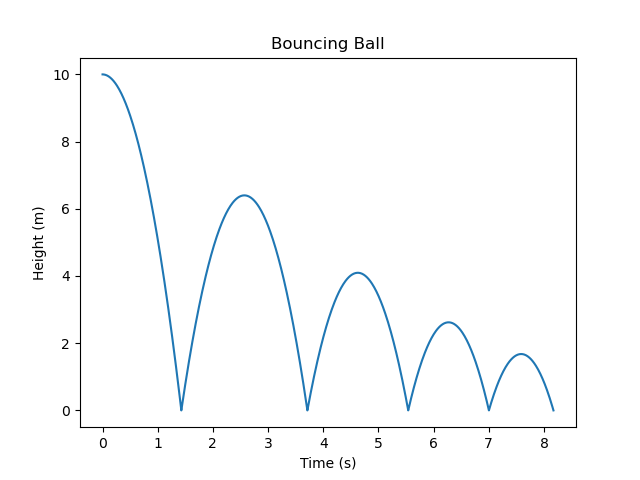
\includegraphics[width=0.75\linewidth]{Figure_1.png}
    \caption{Trajectory of a bouncing ball with varying elasticity}
    \label{fig:placeholder}
\end{figure}

I then wrote a script to model a planet's trajectory around a star - this required an extra variable and introduced coupled equations in my state variable. The third script added a moon, pushing me to develop the state variables for multiple objects within one function. It also marked the point where I started paying attention to tolerance and step size.

Having understood the integrator, I moved on to a simulation that more closely modeled the final product. I decided to trace rays from a source point near a mass to a screen entirely using Newtonian physics. In the initial 2D model, the rays depended solely on $\theta$, restricted from -30 to 30, the angle from the horizontal (the source point and point mass lay on the x-axis). Determining the state values was simple using Newtonian physics, and the two terminal events - hit\_screen and hit\_object - tracked contact with the screen and contact with the mass, respectively.

Each event is a function of the current state of the object we track, and SciPy stops the integration when one of those events hits zero. For example, \texttt{hit\_screen} returns the distance from the screen, and when the integrator calculates that distance to be zero, it stops and moves to the next launch angle.

It is worth clarifying the direction of the light tracing. In reality, light comes from the background (our "screen") and arrives at our eye - the point I call the source is really the observer. Therefore, this simulation actually traces rays backwards, since they travel from the source to the screen. Going backwards, every ray we launch actually reaches the background, and wherever a ray lands is what the observer sees in that direction.

There is one major caveat: in Newtonian gravity, light doesn't actually bend. While working in Newtonian physics, what I traced were not photons but test particles - small masses launched at fixed speeds. Geometrically, they stand in for light rays, but the underlying physics does not actually apply to photons, which is why the trajectories shown are not physically achievable.

After plotting the rays \textbf{(Figure 2)}, having colored the positively angled rays blue and the negative red, I noticed an interesting pattern. Many of the red rays and blue rays ended up on the same point on the screen; therefore, the point observer would see a duplicated image above and below the central mass. This phenomenon closely matches black hole lensing: because of the extreme bending of light, duplicates appear in many simulations. However, the trajectories shown in the diagram are not physically feasible; the mass would have to be extremely large, which would make the rays behave less like Newtonian trajectories and more like GR geodesics. They are shown just to demonstrate a hypothetical.


\begin{figure}[H]
    \centering
    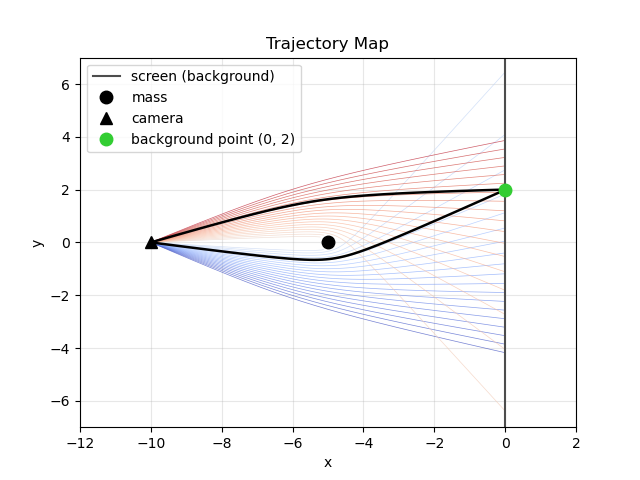
\includegraphics[width=0.75\linewidth]{Figure_2.png}
    \caption{Rays warped around a point mass via Newtonian physics - color based on launch angle}
    \label{fig:placeholder}
\end{figure}
I then built a 3D model, introducing $\phi$ as a parameter alongside $\theta$, so that the rays launch in a cone rather than a fan. Although the geometry was the same, this introduced the issue of interpolation. The points where the rays hit the screen were spaced significantly, raising issues about how I could get a fully visible image in the background. Tracing one ray per pixel is too costly, but luckily the image doesn't really need it - far from the mass, rays land in a smooth pattern, so I could interpolate between the points I actually calculate.

% ============================================================
\section{Phase II — Schwarzschild Geodesics}
\label{sec:schwarzschild}
% Metric -> Christoffels -> geodesic equation. Natural units.
% End on: build-time vs run-time cost; the physics validates itself.
With the general code structure established, I shifted from Newtonian to general relativistic trajectories. The biggest change was in what I was tracing. In Phase I, the test particles had mass, but in general relativity light has no mass; instead, it follows a null geodesic, the straightest path through spacetime. The general structure - plotting code, events - stayed the same; however, the differential equation itself changed. The new ODE was based on the Schwarzschild metric; I used the metric to compute Christoffel symbols, which I then plugged into the equation.

This is the point where SymPy earns its place (\texttt{sp} being SymPy, imported as \texttt{import sympy as sp}). There are 64 Christoffel symbols, and each one is built from the derivatives of metric terms. Working them out by hand is extremely tedious for Schwarzschild, and unmanageable once I added spin. However, SymPy computes them symbolically before any integration happens. Those results are then converted to numerical functions with \texttt{sp.lambdify}, turning a symbolic expression into something NumPy can understand. The expensive symbol work is done once at the very start, and from there the integration only calls the fully compiled functions.

The Schwarzschild matrix is a $4\times4$ diagonal matrix of coordinates ($t$, $r$, $\theta$, $\phi$). I decided to build it as a \texttt{sp.Matrix}, making the four coordinates symbolic but leaving $G$, $M$, and $c$ (the gravitational constant, mass, and speed of light, respectively) as variables with set values. I then computed the Christoffel symbols according to:

\begin{equation}
    \Gamma^{\alpha}_{\ \beta\gamma} = \frac{1}{2} g^{\alpha\delta}
    \left( \frac{\partial g_{\delta\beta}}{\partial x^{\gamma}}
         + \frac{\partial g_{\delta\gamma}}{\partial x^{\beta}}
         - \frac{\partial g_{\beta\gamma}}{\partial x^{\delta}} \right).
    \label{eq:christoffel}
\end{equation}

Here, $\alpha$, $\beta$, $\gamma$, and $\delta$ are indices for $g$, the Schwarzschild matrix. Repeated indices imply summation, so each symbol carries an implicit sum over $\delta$.

With the Christoffel symbols calculated, I defined the trajectory based on the geodesic equation:

\begin{equation}
\frac{d^2x^{\alpha}}{d\lambda^2} + \Gamma^{\alpha}_{\ \beta\gamma}
\frac{dx^{\beta}}{d\lambda}\frac{dx^{\gamma}}{d\lambda} = 0.
\label{eq:geodesic}
\end{equation}

In a way, this is the GR replacement for $F=ma$, with the Christoffel symbols standing in for force. $\lambda$ is an affine parameter - for massive particles, proper time works, but proper time doesn't apply to a light ray. One more condition is needed: the four-velocity must satisfy $g_{\mu\nu}u^{\mu}u^{\nu} = 0$, the null condition. I used this at launch to solve for the time component $u^t$ from the spatial directions I had picked.

Due to the extreme bending of light at impact parameters near the critical value, I decided to launch rays at a logarithmic spacing, clustering rays near the critical impact parameter. This allowed for more interesting phenomena, such as light bending around the black hole multiple times before being ejected from its orbit.

I also added a third event, \texttt{escape\_sphere}, which fires when a ray crosses a large sphere around the black hole. Without it, a ray that misses both the screen and the black hole would keep integrating until it hit its limit.

% ============================================================
\section{Phase III — Kerr-Schild Coordinates}
\label{sec:kerr}
% Boyer-Lindquist rejected; implicit r; simplify dropped; closed-form inverse.
The Schwarzschild geometry provided a good introduction to general relativistic orbits; however, extending to a spinning black hole was not simply a matter of using a more complex matrix. The choice of coordinates matters as much. The Schwarzschild coordinates I had been using have a coordinate singularity at the horizon. For an integrator that follows rays towards the black hole until they are captured, such a setup is fatal. Instead, Kerr-Schild coordinates, which are more Cartesian-like, avoid this problem. As a bonus, I could remove the Jacobian conversion I had needed when working with Schwarzschild black holes.

The Kerr-Schild metric is built on:

\begin{equation}
    g_{\mu\nu} = \eta_{\mu\nu} + f\, l_{\mu} l_{\nu}.
    \label{eq:ks-ansatz}
\end{equation}

Here, $\eta$ is the Minkowski tensor, $f$ is a scalar function, $l$ is a null vector, and $a$ is the spin parameter. I used $a = 0.25$ as the convention. The complication is $r$ - instead of representing linear distance ($\sqrt{x^2+y^2+z^2}$), $r$ is defined as follows:

\begin{equation}
    r^{2} = \tfrac{1}{2}\left[ (R^{2} - a^{2})
        + \sqrt{(R^{2} - a^{2})^{2} + 4a^{2}z^{2}} \right],
    \qquad R^{2} = x^{2} + y^{2} + z^{2}.
    \label{eq:r-closed}
\end{equation}

I decided to leave $r$ explicit rather than as a symbol. While it made the symbolic build slower, it eliminated the additional code needed to incorporate a more complex symbolic value. Surprisingly, at this stage I had to leave behind \texttt{sp.simplify}, which I had been using throughout; instead, I used \texttt{cse} while lambdifying my function to recover efficiency.

\textbf{Figure 3} shows null geodesics traced near the Kerr-Schild black hole. The black hole sits at the origin, with rays launched from $(-50, 0, 0)$ and a screen at $x=30$. Everything is in natural units with $G=c=1$ and $M=0.5$.

\begin{figure}[H]
    \centering
    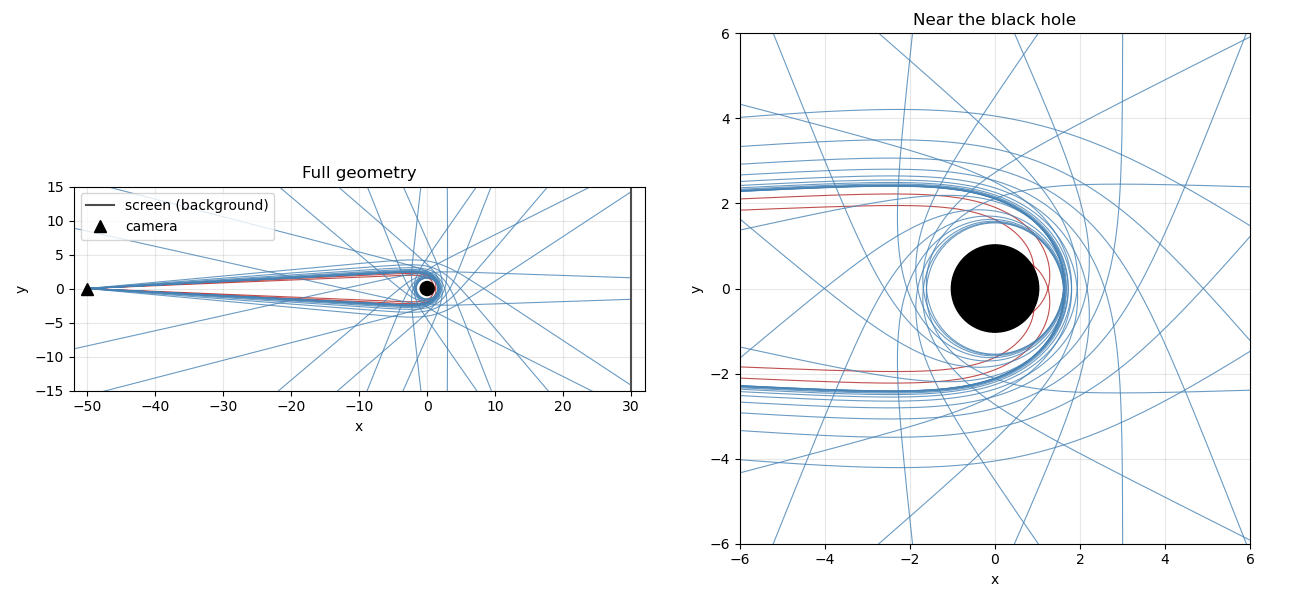
\includegraphics[width=0.75\linewidth]{Figure_3.png}
    \caption{Null geodesics near a Kerr-Schild black hole, shown over the full source-to-screen geometry (left) and zoomed in on the black hole (right). Blue rays escape to the screen; red rays are captured. Rays launched just above the critical impact parameter wind around the black hole before escaping.}
    \label{fig:placeholder}
\end{figure}
% ============================================================
\section{Limitations and Future Work}
\label{sec:limitations}

The simulation has two major limitations: completeness and flexibility.

The script tracks light according to geodesics, but it doesn't account for what happens along the way - intensity, redshift, etc. A real observer would see a different image, shifted in color and brightness, than the simulation shows. There is also no accretion disk present - a real black hole is often seen accompanying an accretion disk, but here, due to the abundance of factors left unaccounted for, the disk is not present.

The second limitation is that many parameters are fixed once the simulation is generated. The spin parameters and observer position are baked into the warp map, and changing either means regenerating the program from scratch.

Natural solutions appear for both. Carrying photon energy with each particle and updating it based on the corresponding forces would let unaccounted effects show, and the existing integrator could support it without changing its structure. Creating $a$ as a symbol and replotting when the user moves the observer position would resolve the second - however, the simulation would be considerably slower.

% ============================================================
\section{Conclusion}
\label{sec:conclusion}

Over three phases, the project went from tracing rays past a point mass with Newtonian gravity to rendering the same through a spinning black hole. Each stage maintained the code's basic framework while replacing the underlying physics: the source-lens-screen geometry survived from the first simulation until the Kerr-Schild black hole, but what changed each time was the differential equation.

The recurring issue was improving efficiency. Filtering nonzero Christoffel symbols prevented the program from lambdifying countless $0$'s for nothing. Abandoning \texttt{sp.simplify} for \texttt{cse} sped up basic computation. Precomputing the warp map moved all of the heavy physics calculation out of the main loop, which is why the result can be viewed in a browser at all.

The final simulation warps any supplied image - a photograph, video, or live webcam feed- as it would appear when lensed by a rotating black hole.
% ============================================================


\end{document}